%=======================================================================
%  Projecting sectoral interactions under climate futures
%=======================================================================
\documentclass[11pt,a4paper]{article}

\usepackage[utf8]{inputenc}
\usepackage[T1]{fontenc}
\usepackage[english]{babel}
\usepackage{amsmath,amssymb,amsthm}
\usepackage{graphicx}
\usepackage{booktabs}
\usepackage{geometry}
\geometry{margin=2.5cm}
\usepackage{natbib}
\bibliographystyle{plainnat}
\usepackage[hidelinks]{hyperref}
\usepackage{float}
\usepackage{tikz}
\usetikzlibrary{arrows.meta,positioning}

\usepackage{authblk}

\title{Projecting sectoral interactions under climate futures}
\author[1]{MARCADET Loïc\thanks{Corresponding author: loic.marcadet@etu.univ-orleans.fr}}
\author[2]{PICARD Tom}
\author[3]{PICAULT Matthieu}
\affil[1]{Nexialog Consulting, France \& Université d'Orléans (LEO), France}
\affil[2]{Nexialog Consulting, France}
\affil[3]{IÉSEG School of Management, France}
\date{\today}

\begin{document}
\maketitle

%=======================================================================
\begin{abstract}
Climate risks are increasingly putting pressure on companies. Not only do they have to consider their direct exposure, but they also have to consider how their value chain will be at risk because of transition costs or physical damage. Redirecting their supply and client flows will be essential to mitigate future risk by buying from less climate-exposed sectors and to meet decarbonization objectives.
Redirected flows mean that sectoral interactions will vary, with natural applications to climate-economy problems such as scope 3 estimation or propagation of carbon costs in the value chain. This paper designs a methodology to project input-output matrices, designed to represent sectoral value chains, under different climate futures. It leverages well-known matrix balancing algorithms to illustrate how the tradeoff between production levels and decarbonization efforts may lead to a more or less successful transition. Applying this process to the EXIOBASE input-output database, we (blablabla)
% TODO: repositionner le niveau d'analyse (sectoriel vs entreprise)
\end{abstract}

%=======================================================================
\section{Introduction}
\label{sec:intro}
%=======================================================================

% Add references

In order to achieve a successful transition, industries are expected not only to make their processes more sustainable but also to consider the footprint of their supply chain. Despite longstanding supplier-client relationships, firms are likely to reduce ties to activities that rely on heavy, carbon-intensive processes. These changes would lead to modified sectoral interactions, with the surge of new flows and a shift in historical demand, which is hard to quantify. Although input-output (I/O) models describe a precise view of the economy and the interactions between sectors, they represent a static view, based on national accounts with a couple of years of delay. On the contrary, climate scenarios, produced mainly thanks to Integrated Assessment Models (IAMs), project economic and climate variables over a long horizon but lack sectoral granularity to better understand the links among the economy. Moreover, value chain data are seldom disclosed by companies, leading to blind spots when evaluating their performance (e.g. scope 3 greenhouse gas emissions) or climate resilience.

% REVISED: "close to today's economy" -> close to today's technology at the
% scenario's output levels (the unchanged-technology projection, Section 2.4).
As a result, this article designs a method to reconcile the two by projecting I/O matrices according to climate scenario assumptions, based on the KRAS algorithm. In this model, the uncertainty between decarbonization success and production levels coherent with scenario narratives drives a rebalancing of the sectoral flows. Calibrating this uncertainty depending on source fiability and sector importance in transition, we obtain matrices conditional to given climate scenarios that anticipate the evolution of sectoral interactions depending on how macroeconomy evolves. KRAS properties allow for coherent I/O rebalancing, to obtain a system that stays as close as possible to today's production technology, scaled to the scenario's output levels, while respecting climate constraints as much as possible. In addition, it handles conflicting constraints due to multiple sources, finding tradeoffs between sector GHG reduction and economic steering according to the uncertainties mentioned earlier. We apply this model to applications relevant for financial institutions, such as value chain emissions estimation and propagation of carbon costs in the value chains.

% TODO: question de recherche explicite

%=======================================================================
\subsection{Related work}
\label{sec:related}
%=======================================================================

\paragraph{IO and EEIO}
\label{sub:eeio}
I/O tables properties make them particularly suitable for footprinting, relying on external physical supply and use accounts. Tables like EXIOBASE incorporate intensities for themes like land use or emissions (that is, accounts per unit of monetary output), that can be multiplied with the transaction flows for a footprint estimation \citep{stadler2018exiobase}. For even better accuracy, hybrid monetary-physical I/O systems have been developed, implementing better integration of lice-cycle assessments and increased price granularity. It allows for a better differentiation of impacts, as done by \cite{tobben2018novel} in the case of biodiversity loss due to palm oils.

\paragraph{Transition risk and value chain emissions}
\label{sub:transition_lit}
This footprinting approach has natural applications in the context of climate risk assessment. Historically, a more important part of the literature focused on transition risk, especially due to carbon taxes. Both \cite{aguilar2023green} and \cite{devulder2020carbon} exploit I/O networks to analyze the transmission of carbon taxations across sectors, respectively in Spain and in the global economy. On the other hand, \cite{fahr2024globalization} study the propagation of physical risks in value chains to evaluate how much GDP is lost compared to direct impacts only. For this, they incorporate projected country-level GDP-at risk estimates under a specific climate scenario to shock simultaneously supply and demand, allowing for substitution between different countries.

\paragraph{Scenarios and input-output}
\label{sub:exogenous}
As these forward-looking shock analyzes still rely on historical I/O flows, recent work focused on how to incorporate scenarios to alter I/O matrices. \cite{de2016scenarios} design a business-as-usual (BAU) scenario, a technological innovation scenario and a towards-2-degree scenario that adds demand shift to the technology improvements to modify EXIOBASE1 and quantify resulting emissions, compared with IAM outputs. They balance the matrix after specifying an exogenous production, demand and value added. Restricting the exogenous trajectories to GDP and demand, \citet{wiebe19} modify the coefficients of specific sectors in EXIOBASE3 to simulate a circular economy scenario adapted to scenarios given by IEA. They compare this with a BAU scenario to assess the impact on global economy and employment. Although the intention of projecting the matrix in a scenario is similar to ours, manual, specific changes are applied to the matrix and do not shock all variables for an evolution consistent with the whole climate scenario narrative. Focusing on the steel sector, \cite{rinaldi2024assessing} introduce new low-carbon activities in the I/O table to evaluate the resulting prices and environmental implications, using different scenarios for market share of steel production routes based on the Green Steel Project.

\paragraph{IAM and I/O}
\label{sub:iam}
Since climate scenarios represent the output of complex IAMs, \citet{lefevre24} review studies aiming at improving interactions between IAMs and I/O models. They argue that in most work, they are connected via a ''soft-linking'' approach, where the output of one model is fed as input into the other. ''Hard-linking'' approaches are scarce, because they interconnect both views and their assumptions in a much more intricate way; availability of models and their detailed results is also a hurdle in the use of forward-looking I/O systems.

\paragraph{Matrix balancing}
\label{sub:balancing_lit}
% TODO: positionnement uniquement (d'ou vient le balancing, dans quelles litteratures
% il est mobilise : mise a jour de tables, reconciliation de comptes nationaux,
% construction de MRIO). La mecanique de RAS et KRAS est presentee en
% Section~\ref{sec:method}, ne pas la repeter ici. References : Stone, Junius &
% Oosterhaven, Temurshoev et al., Lenzen et al.
[should there this be subsection in the literature or it's not the focus?]

\paragraph{Contributions}
% TODO

This paper furthers the literature through several contributions. First, instead of evaluating footprints as a result of the matrix transformations, we design a process where the end decarbonization is the main driver of rebalancing flows. Second, we leverage KRAS for a scalable, automated matrix projection with uncertain climate outcomes. Third, our method results in projected I/O matrices tailored for different climate scenarios. Fourth, we exploit these in illustrative financial applications that consider future value chain dynamics.

The remainder of the article is structured as follows. Section \ref{sec:framework} defines the setting and problem formulation. Section \ref{sec:method} explains the methodology used for the projections, while Section \ref{sec:data} presents the data. We validate algorithmics in Section \ref{sec:validation}, and present results from theoretical experiments in Section \ref{sec:results}. We apply the process to financial applications in Section \ref{sec:applications}. Finally, we discuss the limitations in Section \ref{sec:discussion} and conclude in Section \ref{sec:conclusion}.

%=======================================================================
\section{Framework}
\label{sec:framework}
%=======================================================================

This section introduces the I/O setting, states the accounting identities that any projected system must satisfy, and formulates the projection exercise as a matrix balancing problem.

%-----------------------------------------------------------------------
\subsection{Input-output setting and notations}
\label{sub:setting}
%-----------------------------------------------------------------------

% TODO (not part of this revision): N = 163, n = 7987 is the industry-by-industry
% (ixi) table. The runs use the product-by-product (pxp) table, N = 200, n = 9800,
% solved at aggregated resolutions. Settle on one and update this sentence.
We work in a multi-regional setting. Let $r = 1, \dots, R$ index regions and $g = 1, \dots, N$ index sectors. Region-sector pairs are stacked into a single index $i = (r,g)$, so that all vectors and matrices below belong to a space of dimension $n = R \times N$. In EXIOBASE, $R = 49$ and $N = 163$, hence $n = 7\,987$.

% REVISED: y is not sign-restricted (changes in inventories).
\paragraph{Economic block.}
The observed data are the intermediate flows $Z \in \mathbb{R}^{n \times n}$, where $Z_{ij}$ is the value sold by $i$ to $j$ as an intermediate input, and the final demand $Y \in \mathbb{R}^{n \times f}$, whose $f$ columns are the final demand categories (households, government, gross capital formation, changes in inventories, exports) of each region. We write $y = Y \mathbf{1}_f \in \mathbb{R}^n$ for final demand aggregated over categories, and $Y$ for the disaggregated object. $y$ therefore contains final demand only, and intermediate demand is carried by $Z$; a few of its entries can be negative, since changes in inventories go both ways. Total output is $x \in \mathbb{R}^n_+$ and value added is $v \in \mathbb{R}^n_+$. The two accounting identities are the row balance and the column balance:
\begin{equation}\label{eq:balance}
  x = Z \mathbf{1}_n + y,
  \qquad
  x^\top = \mathbf{1}_n^\top Z + v^\top .
\end{equation}

Normalizing the columns of $Z$ by output gives the technical coefficients $A = Z \hat{x}^{-1}$, where $\hat{x}$ denotes the diagonal matrix built from $x$; $A_{ij}$ is the input from $i$ required per unit of output of $j$. Substituting into
\eqref{eq:balance} yields the Leontief model
\begin{equation}\label{eq:leontief}
  x = A x + y
  \quad \Longleftrightarrow \quad
  x = (I - A)^{-1} y = L y ,
\end{equation}
with $L = (I-A)^{-1}$ the Leontief inverse. The series expansion
$L = I + A + A^2 + \cdots$ gives the usual reading: $A^d$ collects the inputs required at depth $d$ of the supply chain (producing a car requires steel, which requires ore, which requires energy...), so that $L$ aggregates all direct and indirect effects of one
unit of final demand.

\paragraph{Environmental block.}
Environmental extensions are stored in $F \in \mathbb{R}^{q \times n}$, the absolute impact of each region-sector for $q$ stressors. Intensities and multipliers follow as
\begin{equation}\label{eq:env}
  S = F \hat{x}^{-1},
  \qquad
  M = S L ,
\end{equation}
so that $S_{\cdot i}$ is the impact generated per unit of output of $i$ and $M_{\cdot j}$ the total impact, direct and indirect, triggered by one unit of final demand for $j$. The
footprint closes the chain:
\begin{equation}\label{eq:footprint}
  E = M y = S L y = S x \; \in \mathbb{R}^q .
\end{equation}
We use \eqref{eq:footprint} in aggregated form throughout. When the sectoral breakdown is needed, the same quantity is written $S \hat{x} \in \mathbb{R}^{q \times n}$ for the production-based allocation and $M Y \in \mathbb{R}^{q \times f}$ for the allocation to final demand categories; both sum back to $E$, along different dimensions.

% REVISED: the stressor actually used is fossil CO2, not GHG.
Throughout the paper we consider a single stressor, fossil CO$_2$ emissions: combustion, plus the non-combustion emissions of cement and lime production. Biogenic CO$_2$ is excluded, as is conventional in scope accounting, and so are the direct emissions of households, which are recorded outside the production block. We write $s \in \mathbb{R}^n_+$ for the corresponding row of $S$ and $m = s L$ for the corresponding row of $M$; the extension to several stressors is immediate.

\paragraph{Time and scenarios.}
The base year is $t_0 = 2021$ and $T$ denotes the projection horizon. A superscript
$(T,k)$ refers to the value of an object at horizon $T$ under scenario $k$; objects
without a superscript are observed at $t_0$. A prime denotes a projected object produced
by our procedure, so that $Z'$, $A'$, $L'$ and $y'$ are the counterparts of $Z$, $A$, $L$
and $y$ at $(T,k)$.

%-----------------------------------------------------------------------
\subsection{Three levers of the footprint}
\label{sub:levers}
%-----------------------------------------------------------------------

Writing the footprint as $E = S L y$ shows that a scenario can act on it through three
distinct channels. Differencing between $t_0$ and $(T,k)$,
\begin{equation}\label{eq:decomposition}
  \Delta E
  = \underbrace{\Delta S \, L y}_{\text{(1) intensities}}
  + \underbrace{S \, \Delta L \, y}_{\text{(2) production structure}}
  + \underbrace{S L \, \Delta y}_{\text{(3) final demand}}
  + \varepsilon ,
\end{equation}
where $\varepsilon$ collects the interaction terms, as is standard in structural decomposition analysis. Lever (1) is technological: cleaner processes at given output, captured by intensity pathways. Lever (3) is behavioural and commercial: consumption patterns, domestic demand, trade. Lever (2) is the one that the input-output literature usually holds fixed, and the one this paper makes endogenous: input substitution, relocation and circularity all
translate into a change of $A$, hence of $L$. Climate scenarios provide information on (1) and on aggregates that bind (2) and (3), but they say nothing about the individual cells of $A$. Our contribution is to recover $\Delta L$ from that partial information,
using the accounting identities \eqref{eq:balance} and \eqref{eq:leontief} to keep the
system closed.

% REVISED (new paragraph): under the production-oriented closure the total is
% pinned; levers (2) and (3) offset exactly.
\paragraph{What the closure leaves to rebalancing.}
The three levers are not independent once output is imposed. Section~\ref{sub:problem} fixes output at $x^{T,k}$ and recovers final demand as $y' = (I - A')\,x^{T,k}$, so that $L' y' = x^{T,k}$ whatever the projected structure. The footprint then reduces to
\begin{equation}\label{eq:fixed_total}
  E' = S^{T,k} L' y' = S^{T,k} x^{T,k},
  \qquad
  E' - E = \Delta S \, x^{T,k} + S \, \Delta x ,
\end{equation}
which depends on intensities and output only. Under this closure, lever (2) is exactly offset by the induced change in final demand: levers (2) and (3), together with their interaction terms, add up to the output effect, whatever the change in structure. Rebalancing therefore cannot raise or lower the total footprint: it changes how that total is \emph{distributed}, across value chains (the embodied emissions of each sector's purchases, Section~\ref{sub:constraints}) and across final demand categories ($M'Y'$). Those distributions, and not the total, are the outcomes of the method; the total serves as an accounting check.

%-----------------------------------------------------------------------
\subsection{Scenario information as linear constraints}
\label{sub:constraints}
%-----------------------------------------------------------------------

% REVISED: states what is actually used, and why GDP is not a constraint.
We assume that, for a given scenario $k$, we have projections for output per sector $x^{T,k}$, for environmental intensities $S^{T,k}$, and possibly for a set of macroeconomic aggregates that correspond to row or column operations on $Z$. Sectors are additionally assigned decarbonization objectives. Not every macroeconomic aggregate qualifies. GDP, in particular, is not an exact linear aggregate of the cells of $Z$: taxes less subsidies on products, valuation differences and trade with regions outside the table break the identity between GDP and the sum of final demand. Imposing it as a row of $G$ would force the flows to satisfy an identity that does not hold, so we do not use it. In the application, output is the only scenario driver of the margins.

\paragraph{Output as the driver.}
Climate scenarios are usually articulated around production, which is also the variable on which a government can effectively act, through industrial policy, subsidies or carbon pricing. We therefore treat output as the entry point of the scenario into the I/O system, and let the intermediate flows adjust around it.

% REVISED: value added enters through a constant share, not through data.
\paragraph{Balancing $Z$ or balancing $A$.}
Output enters the problem in two distinct ways. First, it is a normalisation: since $x^{T,k}$ is known before balancing, $\hat{x}$ is known too, and the map $Z \mapsto A = Z\hat{x}^{-1}$ is a fixed diagonal rescaling, so that adjusting $Z$ and adjusting $A$ are equivalent problems (as shown by \cite{dietzenbacher2009ras} for RAS). We state the problem on $Z$, since value added,
trade and emission constraints are naturally expressed in levels, and recover $A'$ at the end. Second, output is a constraint on the cells themselves: the column balance in \eqref{eq:balance} requires $\sum_i Z_{ij} = x_j - v_j$, so imposing output jointly with
value added fixes the column sums of $Z$. Lacking value-added projections at the sectoral level, we hold each sector's value-added share at its base-year level, $v^{T,k}_j / x^{T,k}_j = v_j / x_j$. The column sums are then
\begin{equation}\label{eq:colsums}
  w^0_j \;=\; x^{T,k}_j \sum_i A_{ij},
\end{equation}
so that each sector keeps its base-year intermediate input budget per unit of output. The value-added share is implied by this choice rather than used as an input.

% UN Handbook IO: For bi-proportional methods, this problem could be expressed either in terms of technical coefficients or transaction values, as shown by de Mesnard (1994) and Dietzenbacher and Miller  (2009), illustrating that the results are indeed equivalent.

\paragraph{General form.}
Let $z = \mathrm{vec}(Z) \in \mathbb{R}^{n^2}$. The scenario projections we use are linear aggregates of the cells of $Z$, so the constraint set takes the form
\begin{equation}\label{eq:constraints}
  G z = c ,
  \qquad
  G \in \mathbb{R}^{p \times n^2},
  \quad
  c \in \mathbb{R}^p ,
\end{equation}
with one row of $G$ per aggregate: column sums (intermediate purchases) and emission aggregates in our application, and in principle row sums (intermediate sales of a sector), submatrix totals (bilateral trade between two regions) or value-added aggregates. Each target $c_i$ is paired with an uncertainty
$\sigma_i > 0$ measuring how reliable it is, a small $\sigma_i$ denoting a target we are unwilling to violate. The role of these uncertainties is made precise in Section~\ref{sub:kras}.

% REVISED (new paragraph): why the row sums are not imposed.
\paragraph{Row sums are left free.}
We impose the column sums \eqref{eq:colsums} but not the row sums, for two reasons that turn out to be the same. Fixing the intermediate sales of every sector at some $u^0$ pins the total of the embodied emissions defined below:
\begin{equation}\label{eq:rowtrap}
  \sum_j b'_j \;=\; \sum_j \sum_i s_i Z'_{ij} \;=\; \sum_i s_i \sum_j Z'_{ij} \;=\; \sum_i s_i u^0_i ,
\end{equation}
a constant. A uniform ambition $\beta < 1$ is then out of reach by arithmetic: rebalancing can only shuffle emissions between value chains. Fixing the row sums also fixes the answer that the closure of Section~\ref{sub:problem} is meant to produce, since $\sum_j Z'_{ij} = u^0_i$ is exactly $y'_i = x^{T,k}_i - u^0_i$. Leaving the rows free is also the economically natural reading: when buyers move away from carbon-intensive suppliers, those suppliers sell less, and their intermediate sales become an outcome of the projection rather than one of its inputs.

% REVISED: scope wording of the three quantities, and the role of E.
\paragraph{Sectoral emission targets.}
For sector $j$ we distinguish:
\begin{itemize}
  \item \emph{Direct (scope 1) emissions}, $d_j = s_j x_j$. These are additive across
        sectors, $\sum_j d_j$ being total territorial emissions, so they involve no
        double counting. However, with $s$ given by the scenario and $x$ fixed as a hard
        constraint, $d_j$ does not depend on $Z$: a scope 1 target cannot be met by
        rebalancing flows, and only acts as an ex post consistency check.
  \item \emph{Emissions embodied in intermediate purchases},
        $b_j = \sum_i s_i Z_{ij}$, i.e.\ the scope 1 emissions of the direct suppliers
        of $j$, attributed to what $j$ buys from them. In the GHG Protocol vocabulary,
        this covers the location-based scope 2 of $j$ when electricity is bought from
        generators, and the first tier of its upstream scope 3. This quantity reads
        the $j$-th column of $Z$, that is the cells describing the value chain of
        sector $j$, and is \emph{linear} in $z$. It is the object our constraints act
        upon.
  \item \emph{Full upstream emissions}, $b^{\mathrm{up}}_j = \sum_i m_i Z_{ij}$,
        obtained by replacing intensities with multipliers. This measure covers scope 2
        and the whole upstream scope 3 (cradle-to-gate, net of scope 1) but is
        \emph{nonlinear} in $z$, since $m = sL$ itself depends on $A$. It cannot enter
        \eqref{eq:constraints} and is instead evaluated after balancing.
\end{itemize}
Downstream scope 3, such as the use of sold products, has no counterpart in an input-output table and is outside the scope of the method. Neither $b_j$ nor $b^{\mathrm{up}}_j$ is additive across sectors: a tonne emitted by an electricity
producer is counted again in the value chain of every sector buying that electricity, so
$\sum_j b_j$ overstates total emissions. Sectoral targets are therefore imposed sector by
sector. The only additive total is the footprint \eqref{eq:footprint}, which allocates each tonne exactly once; under our closure it is set by the scenario \eqref{eq:fixed_total}, so we use it as a consistency check and report sectoral quantities as outcomes.

A decarbonization objective for sector $j$ with ambition $\beta_j^k \in (0,1]$ is thus
written as the linear target
\begin{equation}\label{eq:decarb}
  \sum_i s_i^{T,k} \, Z'_{ij} \; = \; \beta_j^k \sum_i s_i^{t_0} \, Z_{ij} ,
\end{equation}
appended to \eqref{eq:constraints} with its own uncertainty.

% REVISED: replaces "it will generally not be satisfied exactly".
\paragraph{Reading and reach of the targets.}
Three properties of \eqref{eq:decarb} matter for the results. First, ambition is measured against the base year, so $\beta^k_j = 1$ is not a neutral choice: it holds the embodied emissions of sector $j$ at their $t_0$ level despite output growth, which is a binding and, for a growing sector, demanding constraint. Sectors that a scenario leaves without an objective therefore receive no row in $G$ at all, rather than $\beta = 1$. Second, a target cannot be set where no multiplicative update can reach it. Columns with $b_j = 0$, or whose carbon-carrying suppliers all have zero flows, receive no row; they are counted and reported. Third, with its column sum fixed at $w^0_j$ and only its existing suppliers available (zeros are preserved, Section~\ref{sub:kras}), the embodied emissions of sector $j$ can only lie in the band
\begin{equation}\label{eq:band}
  w^0_j \, \min_{i \,:\, Z^0_{ij} > 0} s^{T,k}_i
  \;\le\; b'_j \;\le\;
  w^0_j \, \max_{i \,:\, Z^0_{ij} > 0} s^{T,k}_i ,
\end{equation}
with $Z^0$ the starting matrix defined in Section~\ref{sub:problem}. A target outside this band is unreachable by arithmetic, whatever the algorithm, and is flagged as such. Inside it, and because the row sums are free, the target is met exactly unless it competes with another constraint on the same cells; that conflict, rather than the target alone, is what the uncertainties arbitrate.

% PENDING DECISION -- enable once the intensity pathway S^{T,k} != S^{t0} is in.
% When intensities fall, part of each target is met by the suppliers'
% decarbonization before any rebalancing. If the pathway alone brings
% sum_i s_i^{T,k} Z^0_ij below the target, the equality would require KRAS to
% raise the embodied emissions of column j, i.e. to source from dirtier
% suppliers. Two readings are possible:
%  (a) keep beta as total ambition and drop such columns from the target set,
%      reporting them as met by technology;
%  (b) measure beta against the counterfactual,
%      sum_i s_i^{T,k} Z'_ij = beta_j sum_i s_i^{T,k} Z^0_ij,
%      so that beta measures effort beyond technology.
% Draft text for (a):
% \paragraph{Targets met by technology.}
% When the intensity pathway alone brings the counterfactual embodied emissions
% $\sum_i s^{T,k}_i Z^0_{ij}$ below the target, imposing \eqref{eq:decarb} as an
% equality would force sector $j$ towards more carbon-intensive suppliers. Such
% columns are removed from the target set and reported as met by technology.

%-----------------------------------------------------------------------
\subsection{The projection problem}
\label{sub:problem}
%-----------------------------------------------------------------------

% REVISED: starting point Z^0, the y' >= 0 cap, E' as an identity, outcomes.
We can now state the exercise. Given an observed matrix $Z$ at $t_0$, a scenario $k$
providing $x^{T,k}$ and $S^{T,k}$, and a set of sectoral objectives \eqref{eq:decarb}, we look for a matrix $Z'$ compatible with $G z' = c$, in a sense weighted by the uncertainties $\sigma_i$, that stays as close as possible to the matrix the scenario implies when nothing but output changes.

\paragraph{Starting point.}
That reference is the unchanged-technology projection
\begin{equation}\label{eq:prior}
  Z^0 = A \, \hat{x}^{T,k},
  \qquad
  u^0 = Z^0 \mathbf{1}_n = A\,x^{T,k},
  \qquad
  w^{0\top} = \mathbf{1}_n^\top Z^0 ,
\end{equation}
which applies base-year technical coefficients to scenario output, and whose column sums are \eqref{eq:colsums}. The observed $Z$ is not a suitable reference, since it no longer matches the scenario's output levels: measuring the distance from $Z$ would count the change of scale as structural change. $Z^0$ is used both as the starting point of the algorithm and as the counterfactual against which every change is measured. Its margins are mutually consistent, $\mathbf{1}^\top u^0 = \mathbf{1}^\top w^0$, so that in the absence of emission targets the balancing returns $Z' = Z^0$, that is $A' = A$, and any deformation of the coefficients is attributable to the targets.

% PENDING DECISION -- enable if the power-mix-consistent prior becomes the default.
% \paragraph{A power-mix-consistent prior.}
% Because $Z^0$ rescales each column by the buyer's growth, every buyer keeps its
% base-year supplier shares, while the scenario projects each power technology
% separately. Under $Z^0$, a technology whose output contracts keeps selling in
% proportion to its buyers' growth, and one whose output expands finds no
% intermediate buyer. We therefore reallocate, inside each column $j$ and within the
% set $P_r$ of power technologies of each supplier region $r$, the purchases
% according to each technology's own growth $g_i = x^{T,k}_i / x_i$:
% \begin{equation}\label{eq:mixprior}
%   Z^{0}_{ij} \;\leftarrow\; Z^{0}_{ij}\, g_i \,
%   \frac{\sum_{h \in P_r} Z^0_{hj}}{\sum_{h \in P_r} Z^0_{hj}\, g_h},
%   \qquad i \in P_r .
% \end{equation}
% Column sums, and the amount each buyer spends in each supplier region, are
% unchanged; only the technology mix of the purchases follows the scenario.

\paragraph{Closure.}
From $Z'$ we recover $A' = Z' \hat{x}^{-1}$, $L' = (I - A')^{-1}$, and we
close the accounting by inverting \eqref{eq:leontief} at the imposed output level,
\begin{equation}\label{eq:closure}
  y' = (I - A') \, x^{T,k} = x^{T,k} - Z' \mathbf{1}_n ,
\end{equation}
which yields a projected final demand consistent with the balanced structure. Two objects must be kept apart: the a priori final demand $y^0 = (I - A)\,x^{T,k} = x^{T,k} - u^0$, implied by base-year technology, and the projected $y'$. Their difference $y' - y^0$ is the final demand displaced by the targets at constant output.

\paragraph{Non-negative final demand.}
The scenario output $x^{T,k}$ is obtained by applying sectoral growth rates to $x$, and does not itself satisfy \eqref{eq:leontief} for any non-negative final demand: wherever the buyers of a sector grow faster than the sector itself, $y^0_i < 0$. With the row sums free, rebalancing can also push a previously positive $y'_i$ below zero, when a supplier gains substituted demand beyond its output. KRAS solves equalities only, so the inequality $y' \ge 0$ is approximated iteratively. After each solve, every row with $y'_i < 0$ receives the additional constraint
\begin{equation}\label{eq:rowcap}
  \sum_j Z'_{ij} = x^{T,k}_i \qquad (\text{i.e. } y'_i = 0),
\end{equation}
with an uncertainty set at the level of the column sums, and the system is solved again, until no row is negative. This heuristic finds a point satisfying $y' \ge 0$, not the least-distorting one that a balancer with inequality constraints would find.

\paragraph{Outcomes.}
By \eqref{eq:fixed_total}, the footprint $E' = S^{T,k} L' y' = S^{T,k} x^{T,k}$ does not depend on $Z'$: it is recomputed ex post as an accounting check, not as a result. The pledges are instead assessed sector by sector, by comparing the realised embodied emissions $b'_j = \sum_i s^{T,k}_i Z'_{ij}$ with their targets \eqref{eq:decarb}. The quantities that rebalancing actually moves are reported alongside: the procurement effort of each sector, i.e.\ the share of its input budget that changes supplier,
\begin{equation}\label{eq:effort}
  \pi_j = \frac{1}{2} \sum_i \left| \frac{Z'_{ij}}{\sum_h Z'_{hj}} - \frac{Z^0_{ij}}{w^0_j} \right| ,
\end{equation}
the change in each sector's intermediate sales $\sum_j Z'_{ij} - u^0_i$, the displaced final demand $y' - y^0$, and, in the regional setting, the share of embodied emissions sourced from other regions. Section~\ref{sec:method} describes the balancing algorithm that delivers $Z'$.

%=======================================================================
\section{Method}
\label{sec:method}
%=======================================================================

%-----------------------------------------------------------------------
\subsection{Background: the RAS algorithm}
\label{sub:ras}
%-----------------------------------------------------------------------

Matrix balancing has a long history in input-output analysis, where it was introduced to update an observed table to a more recent year for which only marginal totals are known. The reference procedure is RAS. Suppose the only available targets are the new row totals
$u \in \mathbb{R}^n$ (intermediate sales of each region-sector) and the new column totals $w \in \mathbb{R}^n$ (intermediate purchases). RAS looks for a solution of the biproportional form
\begin{equation}\label{eq:ras}
  Z' = \hat{\rho} \, Z \, \hat{\gamma} ,
\end{equation}
where $\rho, \gamma \in \mathbb{R}^n_{+}$ are row and column multipliers, obtained by alternately rescaling rows to match $u$, then columns to match $w$, until convergence. The name comes from this decomposition into two diagonal scalings around the original
matrix.

The RAS fixed point is the solution of a well-posed problem: among all matrices satisfying the marginal constraints, it selects the one minimizing the relative entropy to $Z$, so that the adjusted table stays as close as possible to the observed structure in an
information-theoretic sense. It also preserves the zeros of $Z$: a transaction absent from the base year remains absent. Its natural extension to matrices with negative entries, GRAS, splits the matrix into positive and negative parts and scales them separately, preserving signs.

Three features make RAS unsuitable for the projection exercise of
Section~\ref{sub:problem}. First, it requires the targets to be mutually consistent, in particular $\mathbf{1}^\top u = \mathbf{1}^\top w$; when they are not, the alternate
scaling does not converge but cycles between the row step and the column step. Second, RAS only accepts marginal totals, whereas the scenario information of Section~\ref{sub:constraints} takes the form of arbitrary linear aggregates: submatrix totals for bilateral trade, and emission aggregates \eqref{eq:decarb} that read a column
weighted by intensities. Third, all targets are treated as equally reliable, whereas some sectors may be better prepared to transition successfully.

%-----------------------------------------------------------------------
\subsection{The KRAS algorithm}
\label{sub:kras}
%-----------------------------------------------------------------------

% REVISED: two phases and the capped relaxation step, as implemented.
KRAS \citep{lenzen09} lifts these three restrictions while keeping the biproportional underlying principle. It works directly with the general constraint set \eqref{eq:constraints}, $G z = c$, and treats the targets as soft: instead of requiring an exact match, it
allows each target $c_i$ to move within a tolerance set by the uncertainty $\sigma_i$ introduced in Section~\ref{sub:constraints}. The algorithm cycles through the constraints and applies to each one a generalised biproportional update: the cells entering constraint $i$ are rescaled by a factor $r_i$, raised to the power of their coefficient in $G$, so that the realised aggregate $(G z^{(\ell)})_i$ reaches its current target $c_i^{(\ell)}$, positive and negative entries being scaled separately so that signs are preserved. This step reduces to the usual row and column scalings when $G$ only encodes marginals, so RAS is recovered as the special case of KRAS with consistent marginal constraints. In the first phase, the targets are held fixed. If the sweeps stop making progress, which only happens when the constraints conflict, relaxation is switched on: before each update, the target of every constraint with $\sigma_i > 0$ is moved towards its realised value by at most one step,
\begin{equation}\label{eq:kras_relax}
  c_i^{(\ell+1)}
  = c_i^{(\ell)}
  + \mathrm{sgn}\!\left[ (G z^{(\ell)})_i - c_i^{(\ell)} \right]
    \min\!\left( \left| (G z^{(\ell)})_i - c_i^{(\ell)} \right| ,\; \alpha \, \sigma_i \right) ,
  \qquad \alpha \in [0,1] .
\end{equation}
As the step is proportional to $\alpha \sigma_i$, uncertain targets are the ones that are most distorted. Conflicting information is thus reconciled by relaxing the constraints just enough to make the system feasible, and when the targets are consistent the first phase converges and no target is relaxed. The detailed update rules and the pseudo-code are given in
Appendix~\ref{app:kras}.

\paragraph{Limitations.}
KRAS convergence is observed empirically rather than guaranteed like for the original RAS. The choice of the $\sigma_i$ directly drives the result, which is why Section~\ref{sub:uncertainty} focuses on their calibration and reports sensitivity tests. Besides, the
preservation of zeros keeps a coherent economy but has restrictions with regards to transition: a supply relationship absent from the base year cannot open up, so new value chains are not allowed by the algorithm.

%-----------------------------------------------------------------------
\subsection{Calibration of the uncertainty values}
\label{sub:uncertainty}
%-----------------------------------------------------------------------

% TBA : regles de calibration des sigma_i selon la fiabilite de la source et
% l'importance du secteur dans la transition.

%-----------------------------------------------------------------------
\subsection{The projection pipeline}
\label{sub:pipeline}
%-----------------------------------------------------------------------

Figure~\ref{fig:pipeline} summarizes the process, from the raw scenario data to the projected matrix and its outcomes.

% REVISED: starting point Z^0, the y' >= 0 loop, outcomes vs identity check.
\begin{figure}[htbp]
\centering
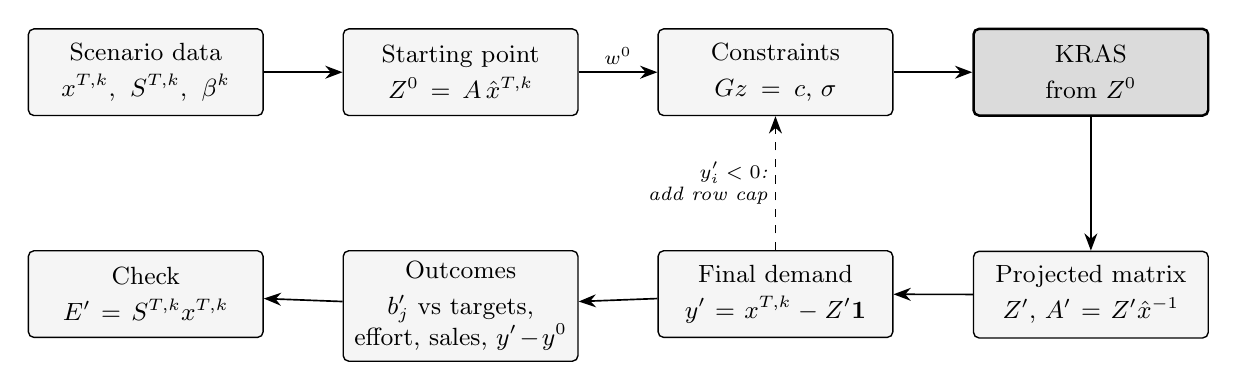
\begin{tikzpicture}[
  font=\small,
  box/.style={draw, rounded corners=2pt, align=center, inner sep=4pt,
              minimum height=1.1cm, text width=2.7cm, line width=0.5pt},
  data/.style={box, fill=black!4},
  algo/.style={box, fill=black!14, line width=0.9pt},
  res/.style={box, fill=black!4},
  ar/.style={-{Stealth[length=2.2mm]}, line width=0.6pt},
  lbl/.style={font=\scriptsize\itshape, inner sep=2.5pt}
]

\node[data] (scen) {Scenario data\\[2pt] $x^{T,k},\; S^{T,k},\; \beta^k$};
\node[data, right=1.0cm of scen] (prior) {Starting point\\[2pt] $Z^0 = A\,\hat{x}^{T,k}$};
\node[data, right=1.0cm of prior] (constr) {Constraints\\[2pt] $Gz = c$, $\sigma$};
\node[algo, right=1.0cm of constr] (kras) {KRAS\\[2pt] from $Z^0$};

\draw[ar] (scen) -- (prior);
\draw[ar] (prior) -- node[lbl, above] {$w^0$} (constr);
\draw[ar] (constr) -- (kras);

\node[res, below=1.7cm of kras] (mat) {Projected matrix\\[2pt] $Z'$, $A' = Z'\hat{x}^{-1}$};
\node[res, below=1.7cm of constr] (dem) {Final demand\\[2pt] $y' = x^{T,k} - Z'\mathbf{1}$};
\node[res, below=1.7cm of prior] (out) {Outcomes\\[2pt] $b'_j$ vs targets,\\ effort, sales, $y'-y^0$};
\node[res, below=1.7cm of scen] (foot) {Check\\[2pt] $E' = S^{T,k}x^{T,k}$};

\draw[ar] (kras) -- (mat);
\draw[ar] (mat) -- (dem);
\draw[ar] (dem) -- (out);
\draw[ar] (out) -- (foot);

% y' >= 0 loop
\draw[ar, dashed] (dem.north) -- node[lbl, left, align=right]
  {$y'_i < 0$:\\ add row cap} (constr.south);

\end{tikzpicture}

\caption{From a scenario to a projected matrix. \\ {\footnotesize Scenario output defines the unchanged-technology starting point $Z^0$ and its column sums; together with the sectoral emission objectives, they form soft constraints with uncertainties. KRAS rebalances the intermediate flows from $Z^0$, and final demand is recovered at the imposed output level. Rows with negative final demand are capped and the system is solved again. The sectoral embodied emissions are compared with their targets, while the total footprint, fixed by output and intensities, serves as an accounting check.}}
\label{fig:pipeline}
\end{figure}

%=======================================================================
\section{Data}
\label{sec:data}
%=======================================================================

\subsection{Input-output data}
\label{sub:exiobase}

EXIOBASE presentation.

\subsection{Climate scenario data}
\label{sub:ngfs}

Many projections are given with units not directly equivalent to EXIOBASE units. We focus on specific variables: Output per sector, output lost per sector, and GDP and macro aggregates. NGFS short term climate scenarios provide these projections in monetary units.
As such, we reuse the YoY evolution of these variables and apply them to the starting point, the EXIOBASE corresponding variable at year $t_0 = 2021$.

\subsection{Sectoral concordance}
\label{sub:concordance}

For this, we perform a matching between the sectors from different sources. The GEM-E3 model, on which NGFS projections are based, includes a mapping towards NACE Rev2 sectors. We conclude the chain with a mapping between NACE Rev2 sectors and EXIOBASE activities.


\begin{figure}[H]
  \centering
  \includegraphics[width=\textwidth]{Figs/proj_exio.png}
  \caption{EXIOBASE macro-aggregates projected with climate variables}
  \label{fig:projex}
\end{figure}

%=======================================================================
\section{Validation}
\label{sec:validation}
%=======================================================================
\begin{figure}[H]
  \centering
  \includegraphics[width=\textwidth]{Figs/kras_history.png}
  \caption{Historical validation}
  \label{fig:history}
\end{figure}
%=======================================================================
\section{Results}
\label{sec:results}
%=======================================================================

TBA

\subsection{Toy example}
\label{sub:toy}

% TBA
\subsection{Large scale experiment}
\label{sub:largescale}

In this section, we rebalance EXIOBASE by focusing on the EU area, and aggregate the imports and exports for the other world regions.

\begin{figure}[H]
  \centering
  \includegraphics[width=\textwidth]{Figs/eu_scenario_ladder.png}
  \caption{Scenario characteristics}
  \label{fig:ladder}
\end{figure}

\begin{figure}[H]
  \centering
  \includegraphics[width=\textwidth]{Figs/eu_sector_scenarios.png}
  \caption{Sector flow adjustments by scenario}
  \label{fig:sectors}
\end{figure}

\begin{figure}[H]
  \centering
  \includegraphics[width=\textwidth]{Figs/eu_flows_baseline.png}
  \caption{Baseline scenario flows (not initial flows)}
  \label{fig:baseline}
\end{figure}

\begin{figure}[H]
  \centering
  \includegraphics[width=\textwidth]{Figs/eu_flows_DAPS.png}
  \caption{"Short term Current Policies"}
  \label{fig:daps}
\end{figure}

\begin{figure}[H]
  \centering
  \includegraphics[width=\textwidth]{Figs/eu_flows_HWTP.png}
  \caption{"Short-term Net Zero"}
  \label{fig:HWTP}
\end{figure}

\subsection{Sensitivity to the ambition $\beta$, the relaxation rate $\alpha$ and the uncertainties $\sigma$}
\label{sub:sensitivity}

NB: This section's example is unrelated to section \ref{sub:largescale}
% TBA

\begin{figure}[H]
  \centering
  \includegraphics[width=\textwidth]{Figs/flows_Z.png}
  \caption{F}
  \label{fig:flows}
\end{figure}


\begin{figure}[H]
  \centering
  \includegraphics[width=\textwidth]{Figs/kras_carbon.png}
  \caption{Decarbonization vs margin deformation with varying uncertainties}
  \label{figs:kc}
\end{figure}

\subsection{Incompatible targets}
\label{sub:incompatible}

% TBA

%=======================================================================
\section{Applications}
\label{sec:applications}
%=======================================================================

\subsection{Value chain emissions application}
\label{sub:scope3}

TBA

\begin{figure}[H]
  \centering
  \includegraphics[width=\textwidth]{Figs/kras_scope3.png}
  \caption{Scope 3}
  \label{fig:s3}
\end{figure}

\subsection{Propagation of carbon costs in the value chain}
\label{sub:carboncosts}

TBA

\begin{figure}[H]
  \centering
  \includegraphics[width=\textwidth]{Figs/gics_cost.png}
  \caption{Costs linked with value chain emissions}
  \label{fa}
\end{figure}

\subsection{(Portfolio allocation with a GHG value chain budget)}
\label{sub:portfolio}

% TBA

%=======================================================================
\section{Discussion and limitations}
\label{sec:discussion}

TBA


%=======================================================================
\section{Conclusion}
\label{sec:conclusion}
%=======================================================================

TBA

%=======================================================================
\appendix

\section{RAS and KRAS details}
\label{app:kras}

\subsection{RAS as an entropy minimisation}

% TBA : programme de minimisation de l'entropie relative sous contraintes marginales,
% conditions d'existence du point fixe, GRAS et le traitement des entrees negatives.

\subsection{KRAS update rules}

% TBA : expression des multiplicateurs par contrainte, separation parties positive
% et negative, gestion des contraintes redondantes.

\subsection{Pseudo-code}

% TBA : algorithme complet, criteres d'arret, complexite par iteration.

\section{Concordance table}
\label{app:concordance}

% TBA

%=======================================================================
\bibliography{references}
%=======================================================================

\end{document}
